\chapter{Installation}

\section{MS-Windows}


To install InVesalius on MS-Windows, simply run the installer program. When a window asking you to confirm the file execution appears, click \textbf{Yes}.

\begin{figure}[!htb]
\centering
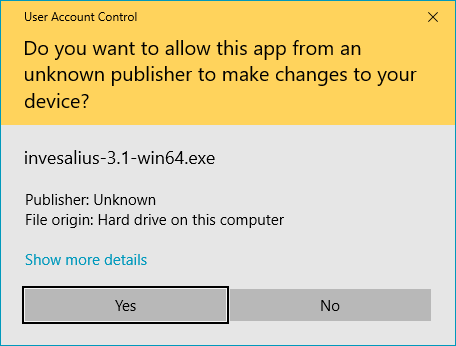
\includegraphics[scale=0.5]{../user_guide_figures/invesalius_screen/installation_exec_en.png}
\end{figure}

\newpage

A new window will ask you to select the language of the installer. Select the language and click \textbf{OK}.

\begin{figure}[!htb]
\centering
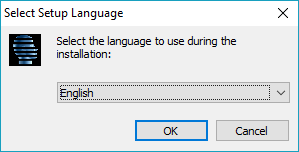
\includegraphics[scale=0.7]{../user_guide_figures/invesalius_screen/installation_select_language_en.png}
\end{figure}
 
\hspace{.2cm}

The Setup installer will appear. Click \textbf{Next}.

\begin{figure}[!htb]
\centering
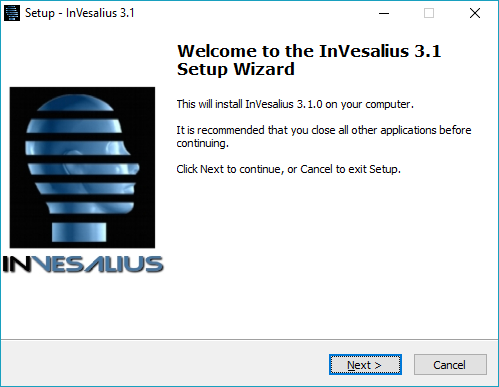
\includegraphics[scale=0.7]{../user_guide_figures/invesalius_screen/installation_welcome_en.png}
\end{figure}

\newpage

Select \textbf{I accept the agreement} and click on \textbf{Next} button.

\begin{figure}[!htb] 
\centering
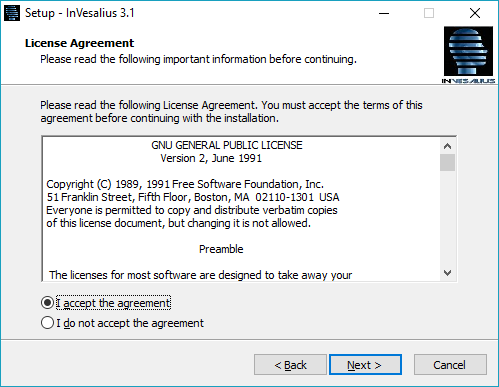
\includegraphics[scale=0.7]{../user_guide_figures/invesalius_screen/installation_license_en.png}
\end{figure}

\hspace{.2cm}

Select the preferred destination for the InVesalius program files, then click \textbf{Next}.

\begin{figure}[!htb]  
\centering
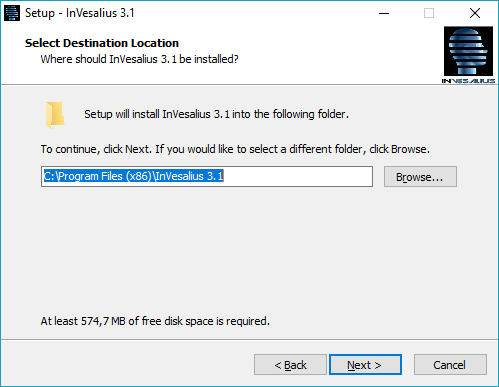
\includegraphics[scale=0.7]{../user_guide_figures/invesalius_screen/installation_folder_en.png}
\end{figure}

\newpage

Click on \textbf{Next}  button.
\begin{figure}[!htb]
\centering
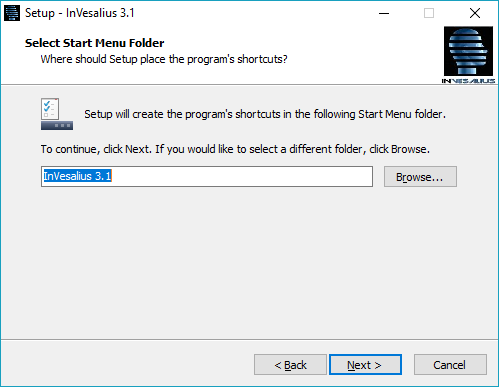
\includegraphics[scale=0.7]{../user_guide_figures/invesalius_screen/installation_program_name_en.png}
\end{figure}

\hspace{.2cm}

Select \textbf{Create a desktop shortchut} and click on \textbf{Next}.

\begin{figure}[!htb]
\centering
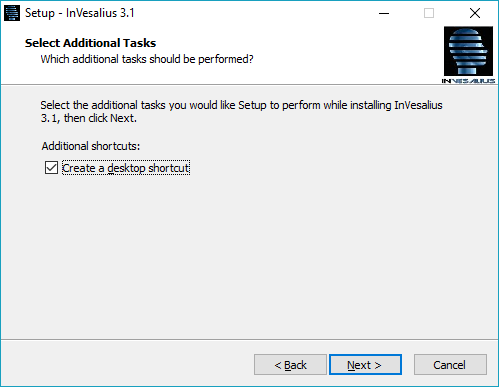
\includegraphics[scale=0.7]{../user_guide_figures/invesalius_screen/installation_desktop_shortcut_en.png}
\end{figure}

\newpage

Click on \textbf{Install} button.

\begin{figure}[!htb]
\centering
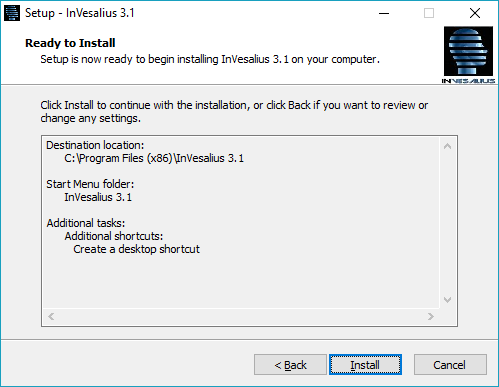
\includegraphics[scale=0.7]{../user_guide_figures/invesalius_screen/installation_resume_en.png}
\end{figure}

\hspace{.2cm}

While the software is being installed, a progress window will appear.

\begin{figure}[!htb]
\centering
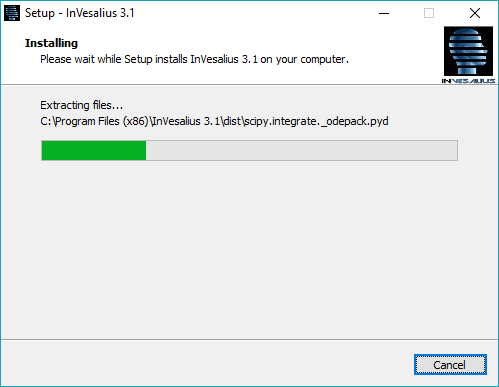
\includegraphics[scale=0.7]{../user_guide_figures/invesalius_screen/installation_progress_en.png}
\end{figure}

\newpage

To run InVesalius after installation, check \textbf{Lauch InVesalius 3.1} and click on \textbf{Finish} button.

\begin{figure}[!htb]
\centering
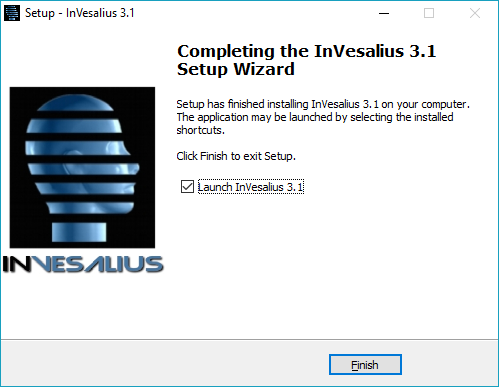
\includegraphics[scale=0.7]{../user_guide_figures/invesalius_screen/installation_finish_en.png}
\end{figure}

\hspace{.2cm}

When being run for the first time, a window will appear to select the InVesalius language. Select the desired language and click \textbf{OK}.

\begin{figure}[!htb]
\centering
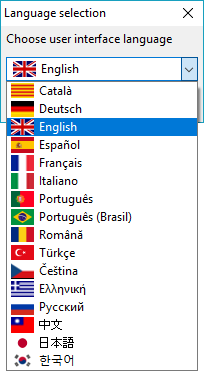
\includegraphics[scale=0.6]{../user_guide_figures/invesalius_screen/invesalius_language_select_en.png}
\end{figure}

\newpage

While InVesalius is loading, the opening window shown below will be displayed.

\begin{figure}[!htb]
\centering
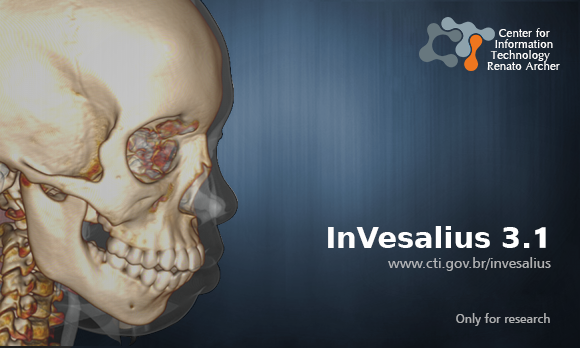
\includegraphics[scale=0.4]{../user_guide_figures/icons/splash_en.png}
\end{figure}

\hspace{.2cm}

The main program window will then open, as shown below.

\begin{figure}[!htb]
\centering
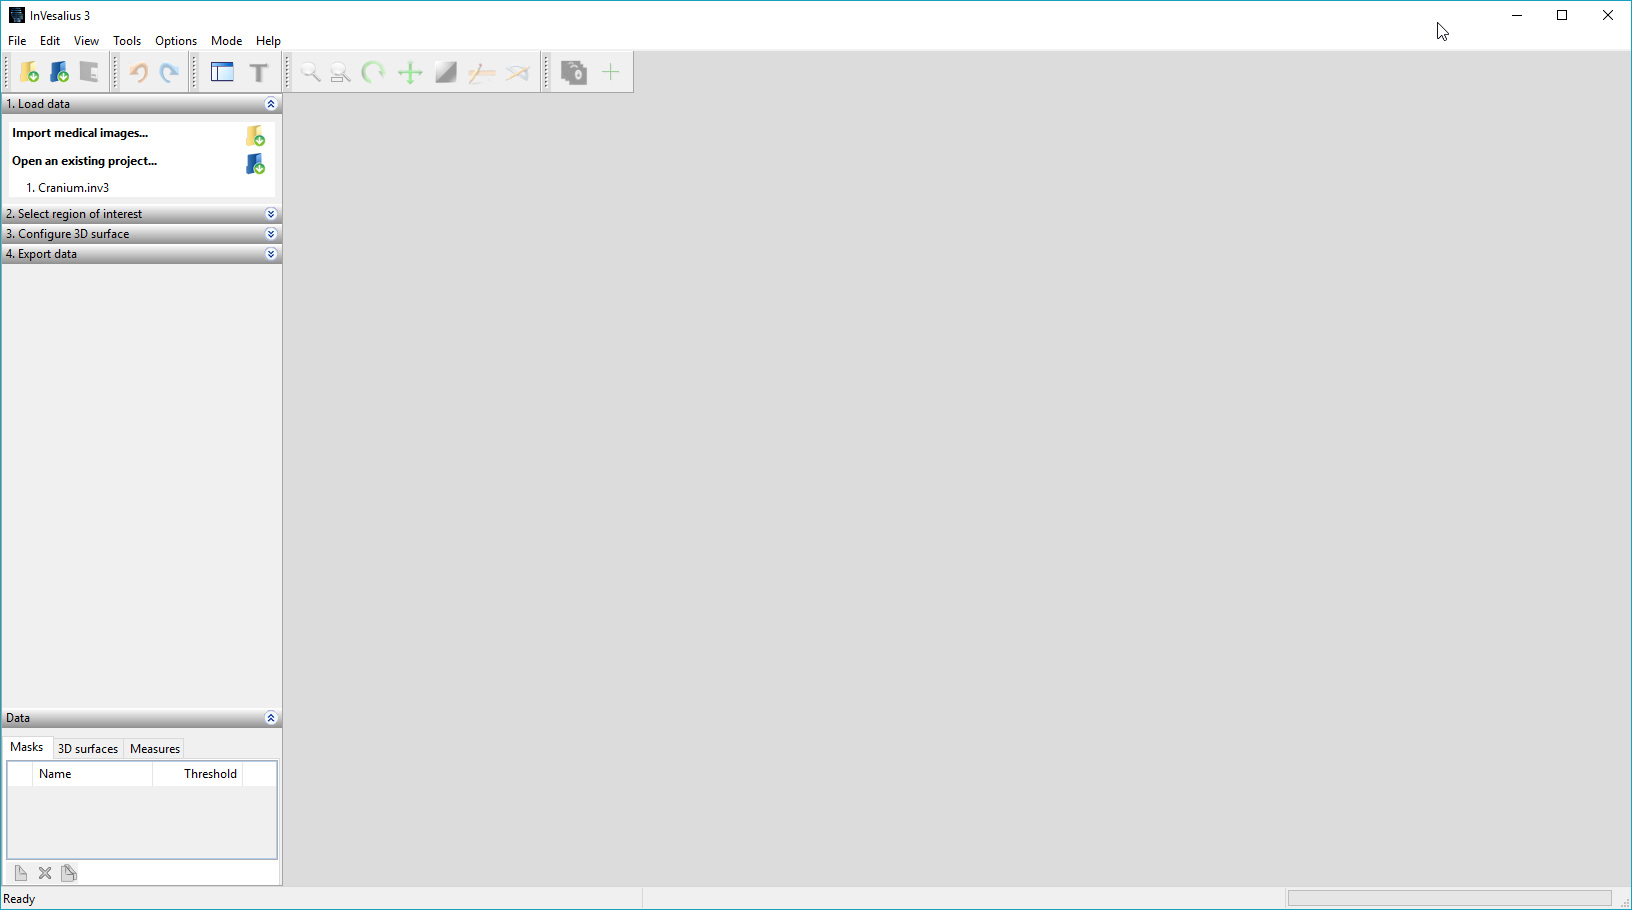
\includegraphics[scale=0.3]{../user_guide_figures/invesalius_screen/main_window_without_project_en.png}
\end{figure}

\section{Mac Os X}

To start the installation on Mac OS X, double-click the installer with the left mouse button to begin installation.

\begin{figure}[!htb]
\centering
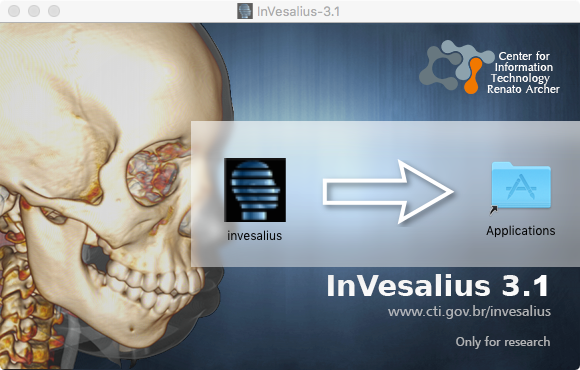
\includegraphics[scale=0.4]{../user_guide_figures/invesalius_screen/mac2.png}
\end{figure}

Hold down the left button on the InVesalius software icon and drag it to the Applications folder. Both are contained in the installer.

%\begin{figure}[!htb]
%\centering
%
\includegraphics[scale=0.4]{../user_guide_figures/invesalius_screen/mac4.png}
%\end{figure}

The software is already installed, just access through the menu.